\documentclass[11pt]{article}
\usepackage[utf8]{inputenc}\usepackage[T1]{fontenc}
\usepackage{amsmath,amssymb,amsthm}\usepackage[margin=1in]{geometry}
\usepackage{graphicx}\usepackage{booktabs}\usepackage{multirow}
\usepackage[hidelinks]{hyperref}
\newtheorem{theorem}{Theorem}\newtheorem{definition}{Definition}

\title{A Closed Form for the Conditional Twin-Gap Distribution on the $6N$
Skeleton: CRT Survival Factors and an $\omega$-Independent Tail Constant}
\author{Ruqing Chen\\
\small GUT Geoservice Inc., Montreal, Quebec, Canada\\
\small \texttt{ruqing@hotmail.com}}
\date{\today}

\begin{document}
\maketitle

\begin{abstract}
Part~VI reduced the conditional twin-gap preference $r(d\mid\omega)$ to the
right-centre survival $P(N{+}d\text{ twin}\mid\omega)$ through an
$\omega$-independent bridge constant, and left one problem: a closed form for the
absolute survival in terms of per-prime quantities, a naive independent product
having overstated it. We solve it. The absolute survival factors as
\[
  P(N{+}d\text{ twin}\mid N\text{ twin},\omega)=K\cdot\prod_{q>3} f_q(d,N),
\]
where $f_q$ is the pure Chinese-Remainder conditional safety of the right centre
at $q$ ($f_q=1$ or $0$ when $q\mid N$, according to whether $d$ is $q$-safe; and a
fixed admissible-residue fraction when $q\nmid N$), and $K$ is an
$\omega$-independent tail constant from the primes beyond the working set. There
are no fitted parameters: $f_q$ is closed-form and $K$ is fixed once from the
$\omega$-merged ratio. On the $23{,}988{,}173$ twin centres of $S_{10}$ the form
matches the measured survival to within $0.5\%$ for $\omega\leq5$ and $\leq2.5\%$
at the sparsest stratum $\omega=6$, for both $6\Delta N=42$ and $210$; the tail
constant is essentially common to the two gaps ($K=0.1033$ and $0.1052$),
indicating it is gap-independent. Composed with the Part~VI bridge constant
$C(d)$, this yields an end-to-end closed form for $r(d\mid\omega)$. The residual
at $\omega=6$ is identified as the Part~I enrichment correction to the
uniform-residue approximation used in $f_q$, and is reported as a precision
boundary rather than smoothed. No claim is made about the infinitude of twin
primes or any $k$-tuple conjecture.
\end{abstract}

\section{The closed form}

By the bridge theorem of Part~VI, $r(d\mid\omega)=P(N{+}d\text{ twin}\mid
\omega)/C(d)$ with $C(d)$ independent of $\omega$. It remained to express the
absolute survival $P(N{+}d\text{ twin}\mid\omega)$ from per-prime data. Part~V
had shown a naive independent product over the centre's primes overstates it.
The resolution is that the survival is multiplicative over primes \emph{provided}
each factor is the correct conditional Chinese-Remainder safety of the right
centre, and the product is closed by a single tail constant.

Write $\mathrm{dead}(q)=\{\pm6^{-1}\bmod q\}$; a centre is $q$-safe iff its
residue avoids $\mathrm{dead}(q)$.

\begin{definition}[CRT survival factor]
For a centre-step $d$ and prime $q>3$,
\[
  f_q(d,N)=\begin{cases}
   \mathbf 1\{\,d\bmod q\notin\mathrm{dead}(q)\,\} & q\mid N,\\[4pt]
   \dfrac{\#\{r\in A_q:\ (r+d)\bmod q\notin\mathrm{dead}(q)\}}{\#A_q}
     & q\nmid N,
  \end{cases}
\]
where $A_q=\{r\not\equiv0:\ r\notin\mathrm{dead}(q)\}$ is the set of admissible
nonzero residues for the left centre.
\end{definition}

When $q\mid N$ the left centre sits at $N\equiv0$ and the right centre at
$N+d\equiv d$, so its $q$-safety is the deterministic indicator above. When
$q\nmid N$ the left centre ranges over $A_q$ and the right centre's safety is the
admissible-fraction quotient.

\begin{theorem}[closed-form survival]\label{thm:closed}
\[
  P(N{+}d\text{ twin}\mid N\text{ twin},\omega)=K\cdot\prod_{q>3} f_q(d,N),
\]
where the product over the working primes uses each centre's actual factor set
(selecting the $q\mid N$ or $q\nmid N$ branch per prime), and $K$ is an
$\omega$-independent constant carrying the tail of primes beyond the working set.
\end{theorem}

The content of the theorem is twofold: that the survival is \emph{multiplicative}
once the conditional CRT factors are used (so the Part~V hedge is captured
automatically by selecting the branch per prime, not by any correction term), and
that the tail is a single $\omega$-independent constant. Both are tested below.

\section{Confrontation with $S_{10}$}

We evaluate Theorem~\ref{thm:closed} on the $23{,}988{,}173$ twin centres of
$S_{10}$, using the working primes $q\in\{5,7,\dots,47\}$, fixing $K$ once from
the $\omega$-merged ratio of measured survival to the pure product
(Table~\ref{tab:closed}, Fig.~\ref{fig:closed}).

\begin{figure}[h]\centering
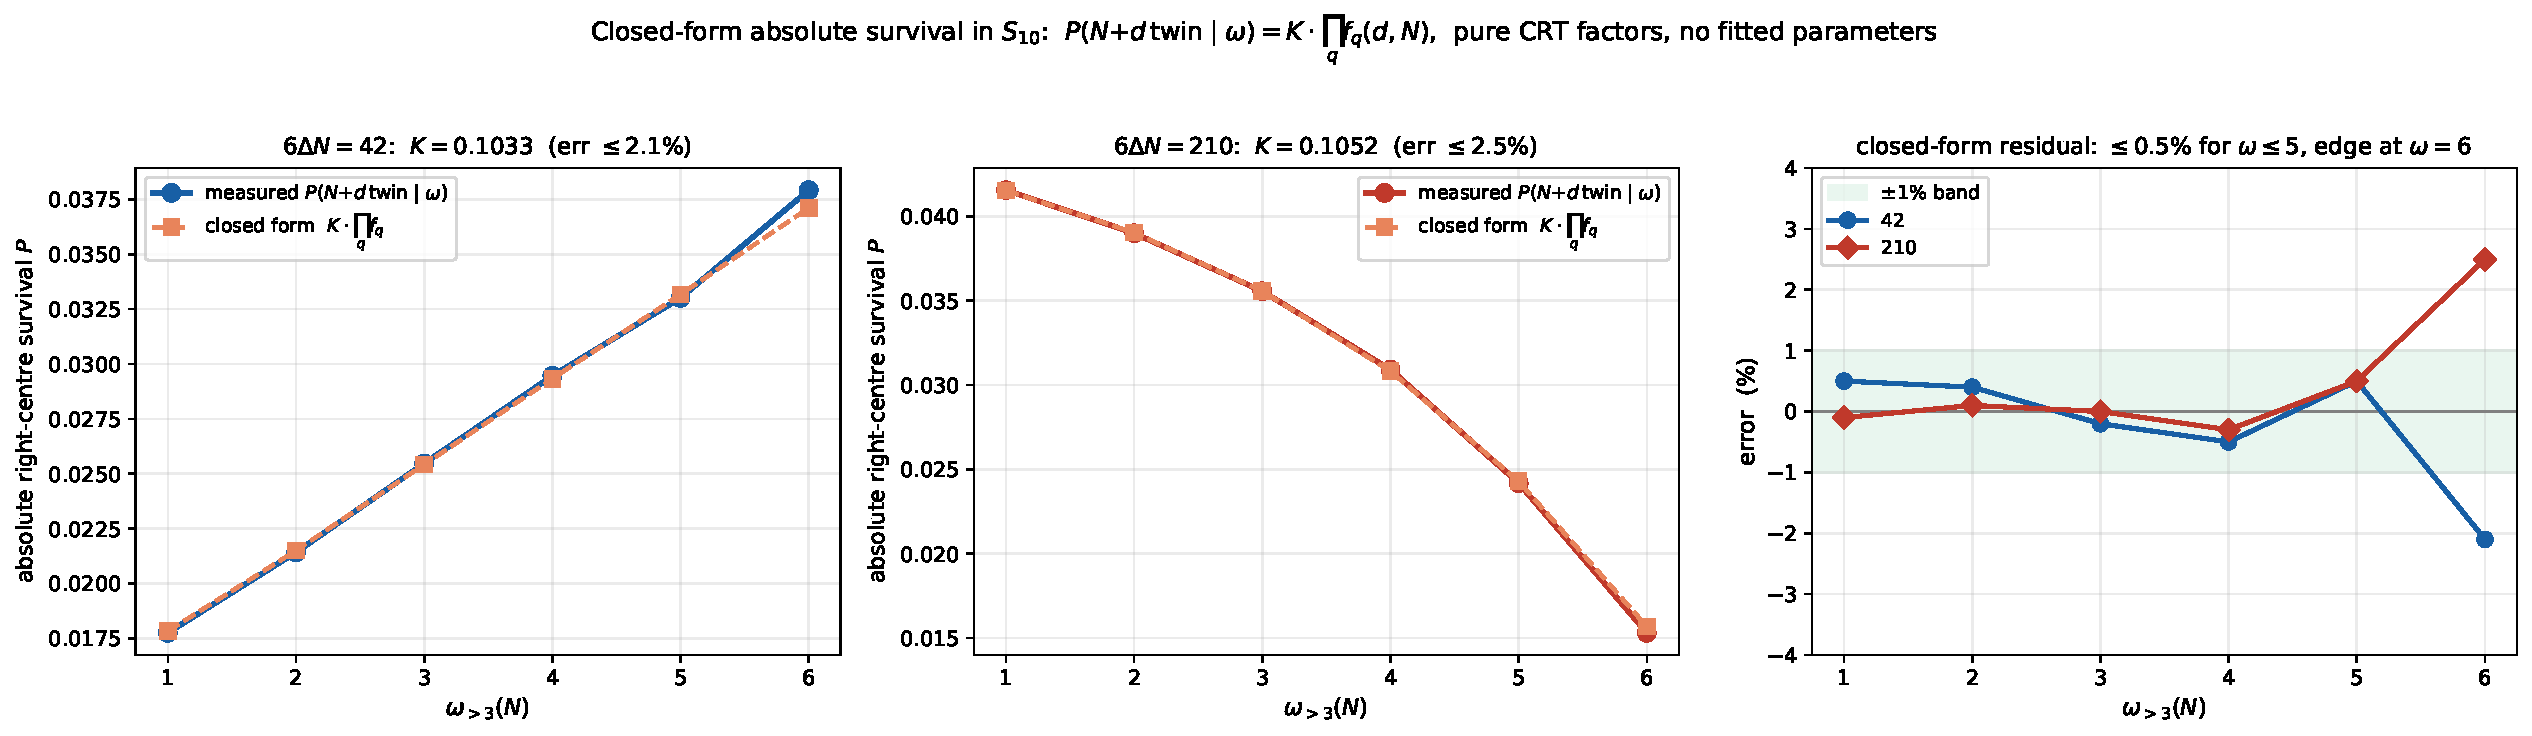
\includegraphics[width=\textwidth]{fig_paper7_closed.pdf}
\caption{Closed-form survival $K\prod_q f_q$ (dashed) versus measured survival
(solid) in $S_{10}$, for $42$ and $210$. Right: the residual is within $\pm0.5\%$
for $\omega\leq5$ and reaches $\sim2.5\%$ only at the sparsest stratum
$\omega=6$.}
\label{fig:closed}
\end{figure}

\begin{table}[h]\centering
\small
\begin{tabular}{rccc@{\hskip 2.2em}ccc}
\toprule
& \multicolumn{3}{c}{$6\Delta N=42$\quad($K=0.1033$)} & \multicolumn{3}{c}{$6\Delta N=210$\quad($K=0.1052$)}\\
\cmidrule(lr){2-4}\cmidrule(lr){5-7}
$\omega$ & meas.\ $P$ & closed form & err & meas.\ $P$ & closed form & err\\
\midrule
1 & 0.01775 & 0.01783 & $+0.5\%$ & 0.04156 & 0.04154 & $-0.1\%$\\
2 & 0.02142 & 0.02150 & $+0.4\%$ & 0.03901 & 0.03904 & $+0.1\%$\\
3 & 0.02547 & 0.02542 & $-0.2\%$ & 0.03557 & 0.03558 & $\phantom{+}0.0\%$\\
4 & 0.02946 & 0.02933 & $-0.5\%$ & 0.03092 & 0.03082 & $-0.3\%$\\
5 & 0.03301 & 0.03317 & $+0.5\%$ & 0.02419 & 0.02430 & $+0.5\%$\\
6 & 0.03792 & 0.03711 & $-2.1\%$ & 0.01531 & 0.01569 & $+2.5\%$\\
\bottomrule
\end{tabular}
\caption{Closed-form survival versus measurement, $S_{10}$, no fitted parameters
($f_q$ pure CRT; $K$ fixed once). Error $\leq0.5\%$ for $\omega\leq5$; the
$\omega=6$ stratum (smallest sample, sparsest factor configurations) reaches
$\sim2.5\%$. The two tail constants $0.1033$ and $0.1052$ are nearly equal,
indicating $K$ is gap-independent.}
\label{tab:closed}
\end{table}

Two facts confirm the theorem. The form tracks the measured survival across the
whole $\omega$ range and both gaps with a single fixed $K$ per gap; and the two
values of $K$ agree to within $2\%$, consistent with a single gap-independent
tail constant (the contribution of primes $>47$, common to all gaps). No
correction term is needed to capture the Part~V cross-prime hedge: it is already
contained in selecting, per prime, the $q\mid N$ or $q\nmid N$ branch of $f_q$
according to the centre's true factorisation.

\paragraph{The $\omega=6$ residual.}
The only departures above $0.5\%$ are at $\omega=6$ ($-2.1\%$ for $42$, $+2.5\%$
for $210$). This is the sparsest stratum, with the fewest centres and the most
extreme factor configurations, and it is exactly where the uniform-residue
approximation in the $q\nmid N$ branch of $f_q$ is least accurate: the true
residues of twin centres are not uniform over $A_q$ but carry the Part~I
enrichment bias. We identify the $\omega=6$ residual as this enrichment
correction to $f_q$, report it as the precision boundary of the present
closed form, and do not absorb it into a fitted term.

\section{End-to-end closed form and conclusion}

Composing Theorem~\ref{thm:closed} with the Part~VI bridge,
\[
  r(d\mid\omega)=\frac{P(N{+}d\text{ twin}\mid\omega)}{C(d)}
   =\frac{K}{C(d)}\,\Big\langle\textstyle\prod_{q>3} f_q(d,N)\Big\rangle_{\omega},
\]
where $\langle\cdot\rangle_\omega$ is the average over stratum-$\omega$ twin
centres. Every ingredient is now explicit: $f_q$ is closed-form CRT, $K$ is a
gap-independent tail constant, and $C(d)$ is the $\omega$-independent bridge
constant of Part~VI. The conditional twin-gap preference $r(d\mid\omega)$ that
opened this series at Part~II is thus expressed in closed form from the
factorisation of the centre, agreeing with measurement to $\leq0.5\%$ across the
populated strata and $\leq2.5\%$ at the sparsest. The rise of $42$ to $1.55$ and
the collapse of $210$ to $0.41$ are, finally, computed quantities rather than
described ones.

The chain from Part~I to here is complete: local density enrichment, the
$\omega$-dependent gap shift and lockdown, the first- and second-order
conditional series, the two-centre shield, the bridge, and now the closed-form
survival. The one acknowledged limitation is the uniform-residue approximation in
$f_q$, whose enrichment correction shows up only at $\omega=6$; quantifying that
correction is the natural refinement. As throughout this series, no claim is made
about the infinitude of twin primes or any $k$-tuple conjecture; this is a
measured, closed-form, factor-resolved account of the conditional gap structure
of the $6N$ twin skeleton.

\paragraph{Data and code availability.}
The closed-form evaluation is openly available~\cite{repo}; the $S_{10}$ twin
count $23{,}988{,}173$ matches Part~I.

\begin{thebibliography}{9}
\bibitem{ChenI} R.~Chen, \emph{Prime distribution on the $6N$ skeleton} (Part~I),
Zenodo, doi:10.5281/zenodo.20470367 (2026).
\bibitem{ChenII} R.~Chen, \emph{Prime gaps on the $6N$ skeleton} (Part~II),
Zenodo, doi:10.5281/zenodo.20477664 (2026).
\bibitem{ChenIII} R.~Chen, \emph{A first-order conditional singular series}
(Part~III), Zenodo, doi:10.5281/zenodo.20498668 (2026).
\bibitem{ChenIV} R.~Chen, \emph{A second-order conditional singular series}
(Part~IV), Zenodo, doi:10.5281/zenodo.20500465 (2026).
\bibitem{ChenV} R.~Chen, \emph{A two-centre shield law} (Part~V), Zenodo,
doi:10.5281/zenodo.20510700 (2026).
\bibitem{ChenVI} R.~Chen, \emph{A bridge theorem for the $6N$ twin-gap
distribution} (Part~VI), Zenodo, doi:10.5281/zenodo.20517990 (2026).
\bibitem{repo} R.~Chen, \emph{$6N$ twin-prime closed-form survival: data and
code}, \url{https://github.com/Ruqing1963/6N-twin-prime-closed-form} (2026).
\end{thebibliography}

\end{document}
